\newpage

\appendix
\section{Appendices}



\section{Box-plot of jump penalties}
\label{appendix:box_plot}

\begin{figure}[H] 
    \centering
    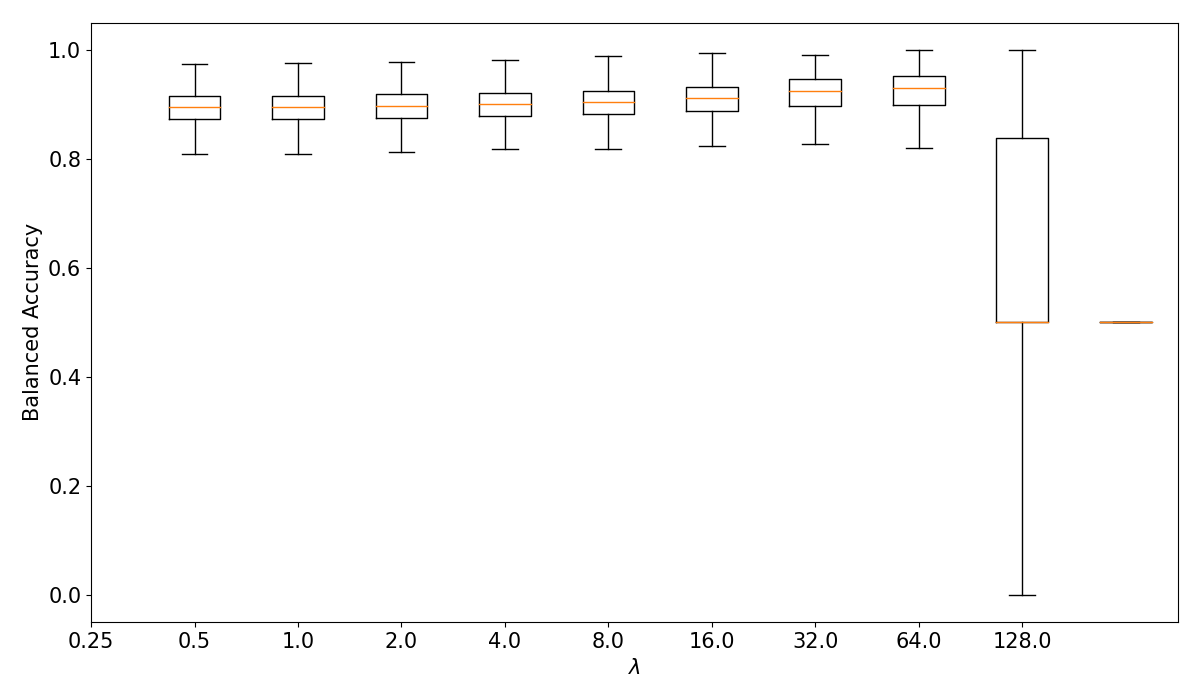
\includegraphics[width=1\textwidth]{analysis/model_convergence/images/jump_penalties_box.png}
    \caption[Boxplot hypertuning the jump penalizer $\lambda$]{Boxplot hypertuning the jump penalizer $\lambda$.}
    %\label{fig:jump_penalties}
\end{figure}

\section{Simulation results}
\label{appendix:model_convergence}

\begin{figure}[H] 
    \centering
    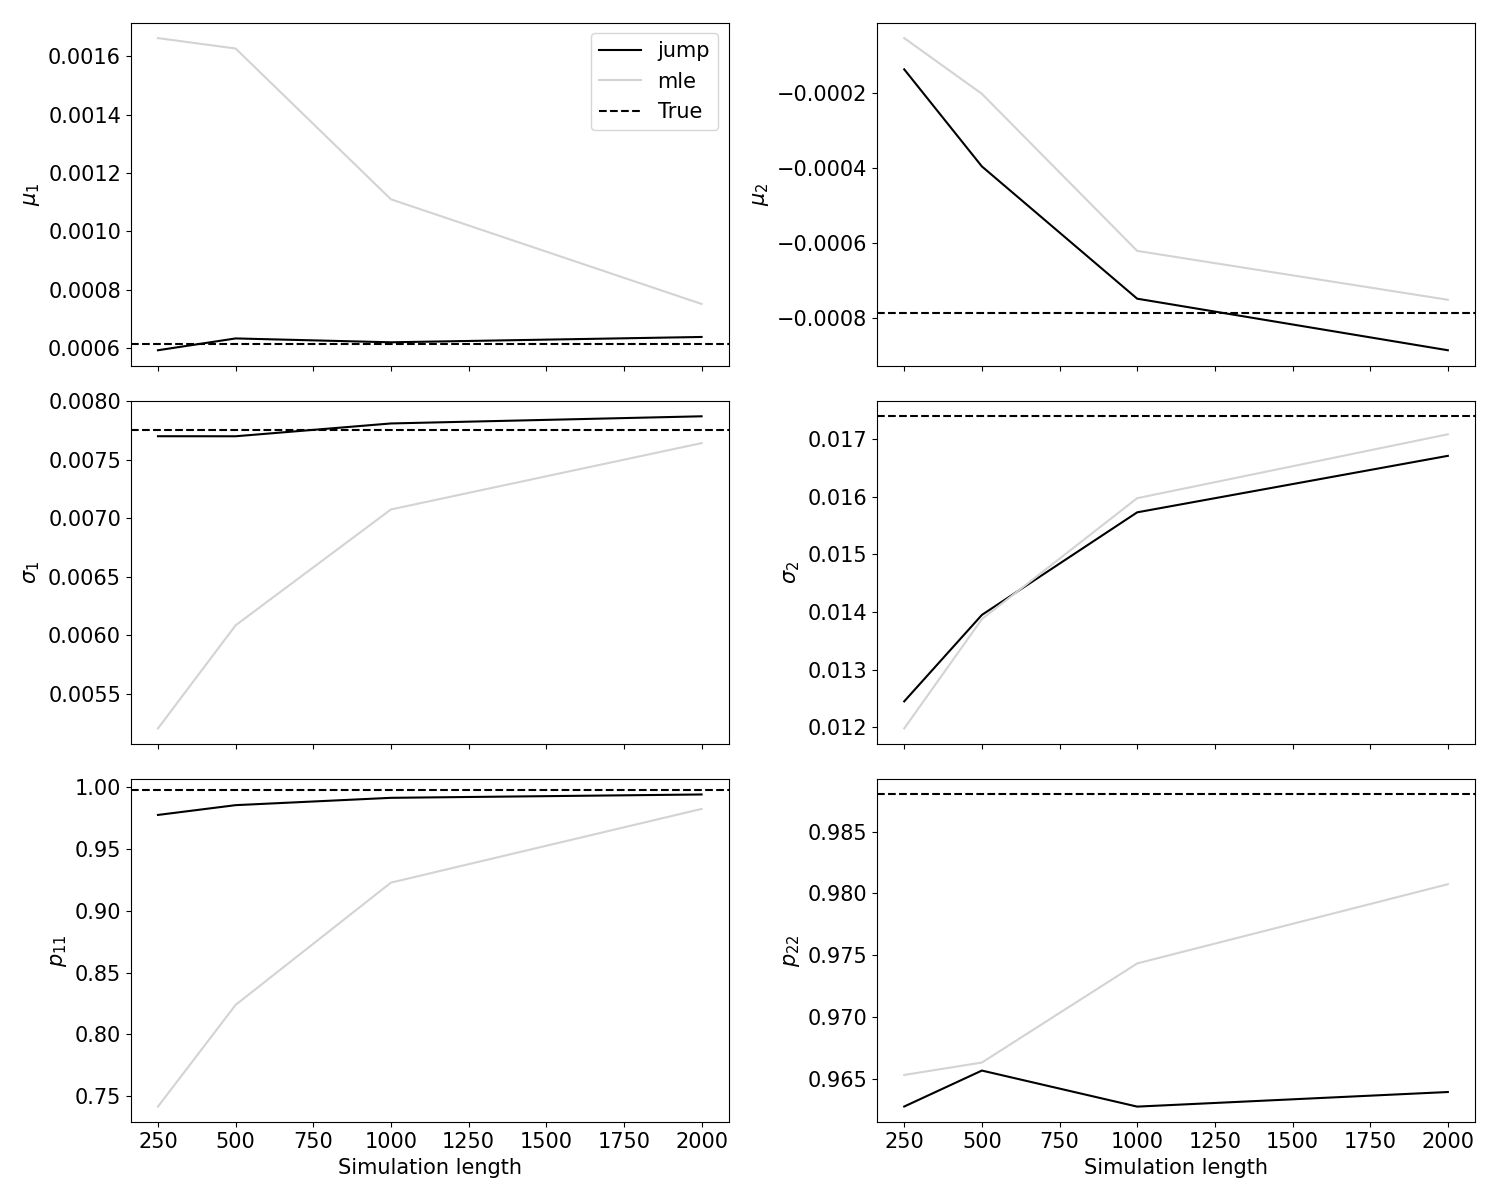
\includegraphics[width=1\textwidth]{analysis/model_convergence/images/simulation_normal.png}
    \caption[Plot of the \mle and \jump parameters, from conditional Gaussian distribution, showing the convergence to the true values]{Plot of the \mle and \jump parameters from conditional Gaussian distributions. The estimates show the models' convergence towards true values as a function of simulation length. Results are based on 1000 simulations.}
    \label{fig:jump_normal}
\end{figure}

\begin{figure}[H] 
    \centering
    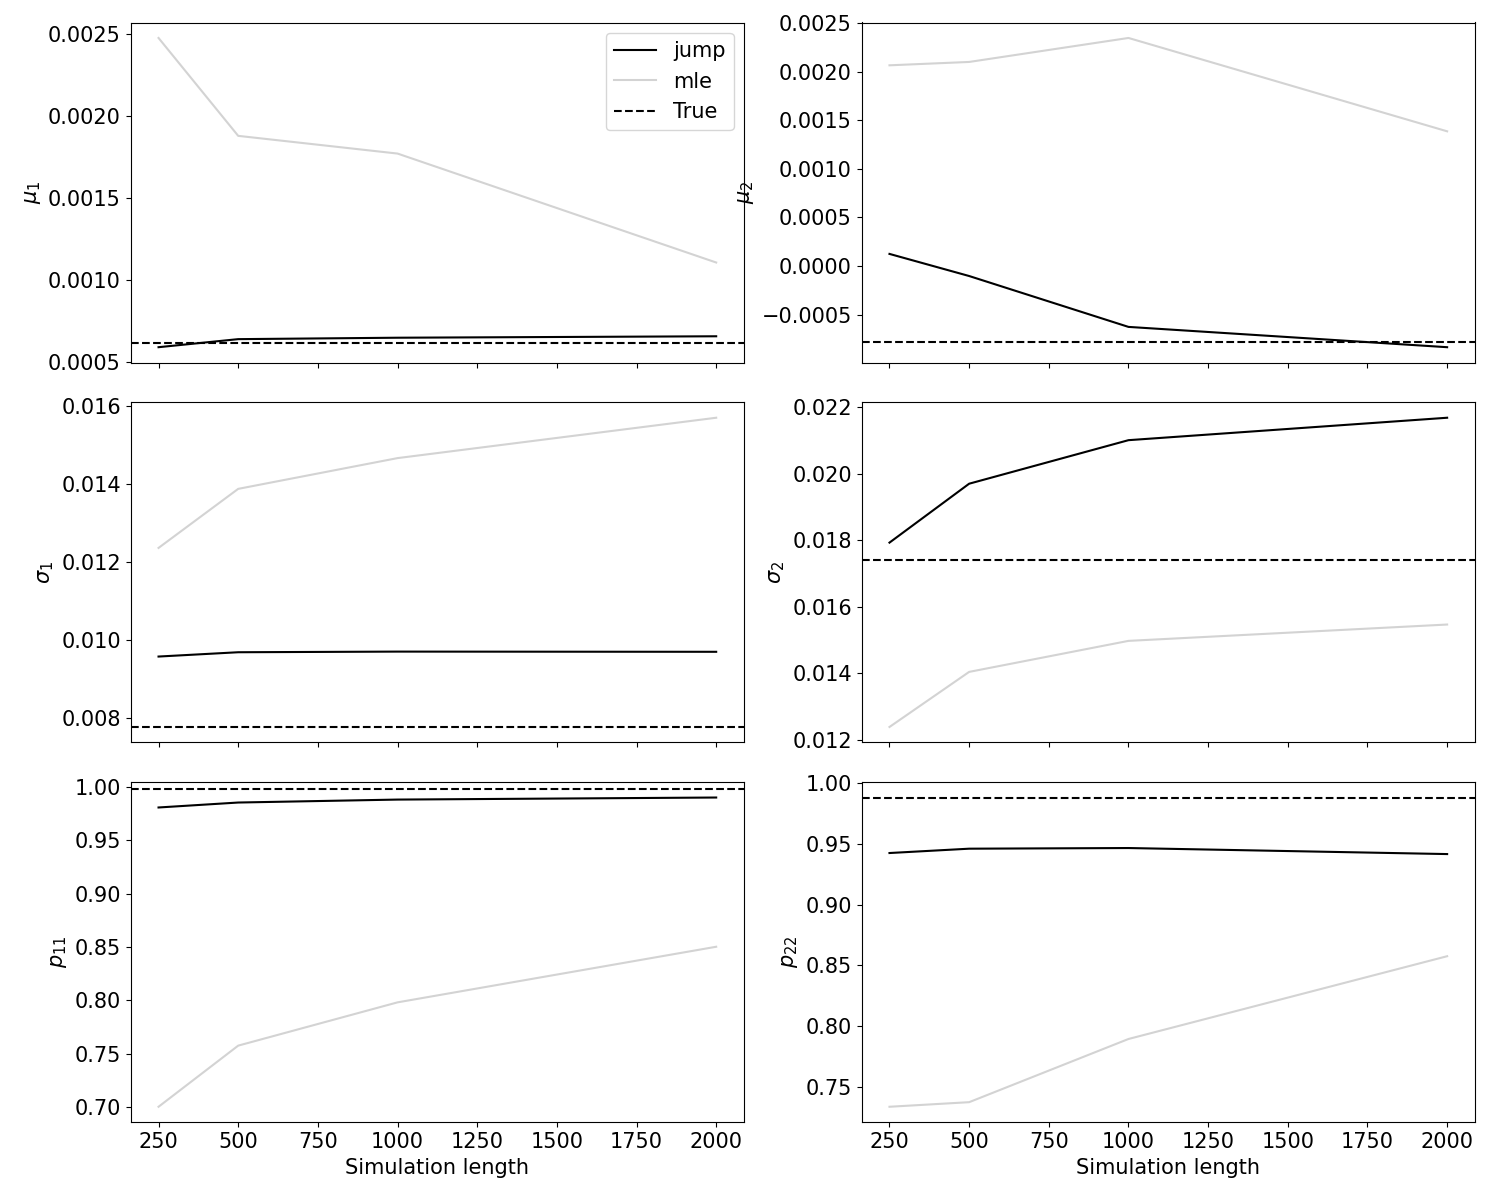
\includegraphics[width=1\textwidth]{analysis/model_convergence/images/simulation_t.png}
    
    \caption[Plot of the \mle and \jump parameters, from conditional t-distributions with five degrees of freedom, showing the convergence to the true values]{Plot of the \mle and \jump parameters from conditional t-distributions with five degrees of freedom. The estimates show the models' convergence towards true values as a function of simulation length. Results are based on 1000 simulations.}
    \label{fig:jump_t}
\end{figure}

\begin{figure}[H] 
    \centering
    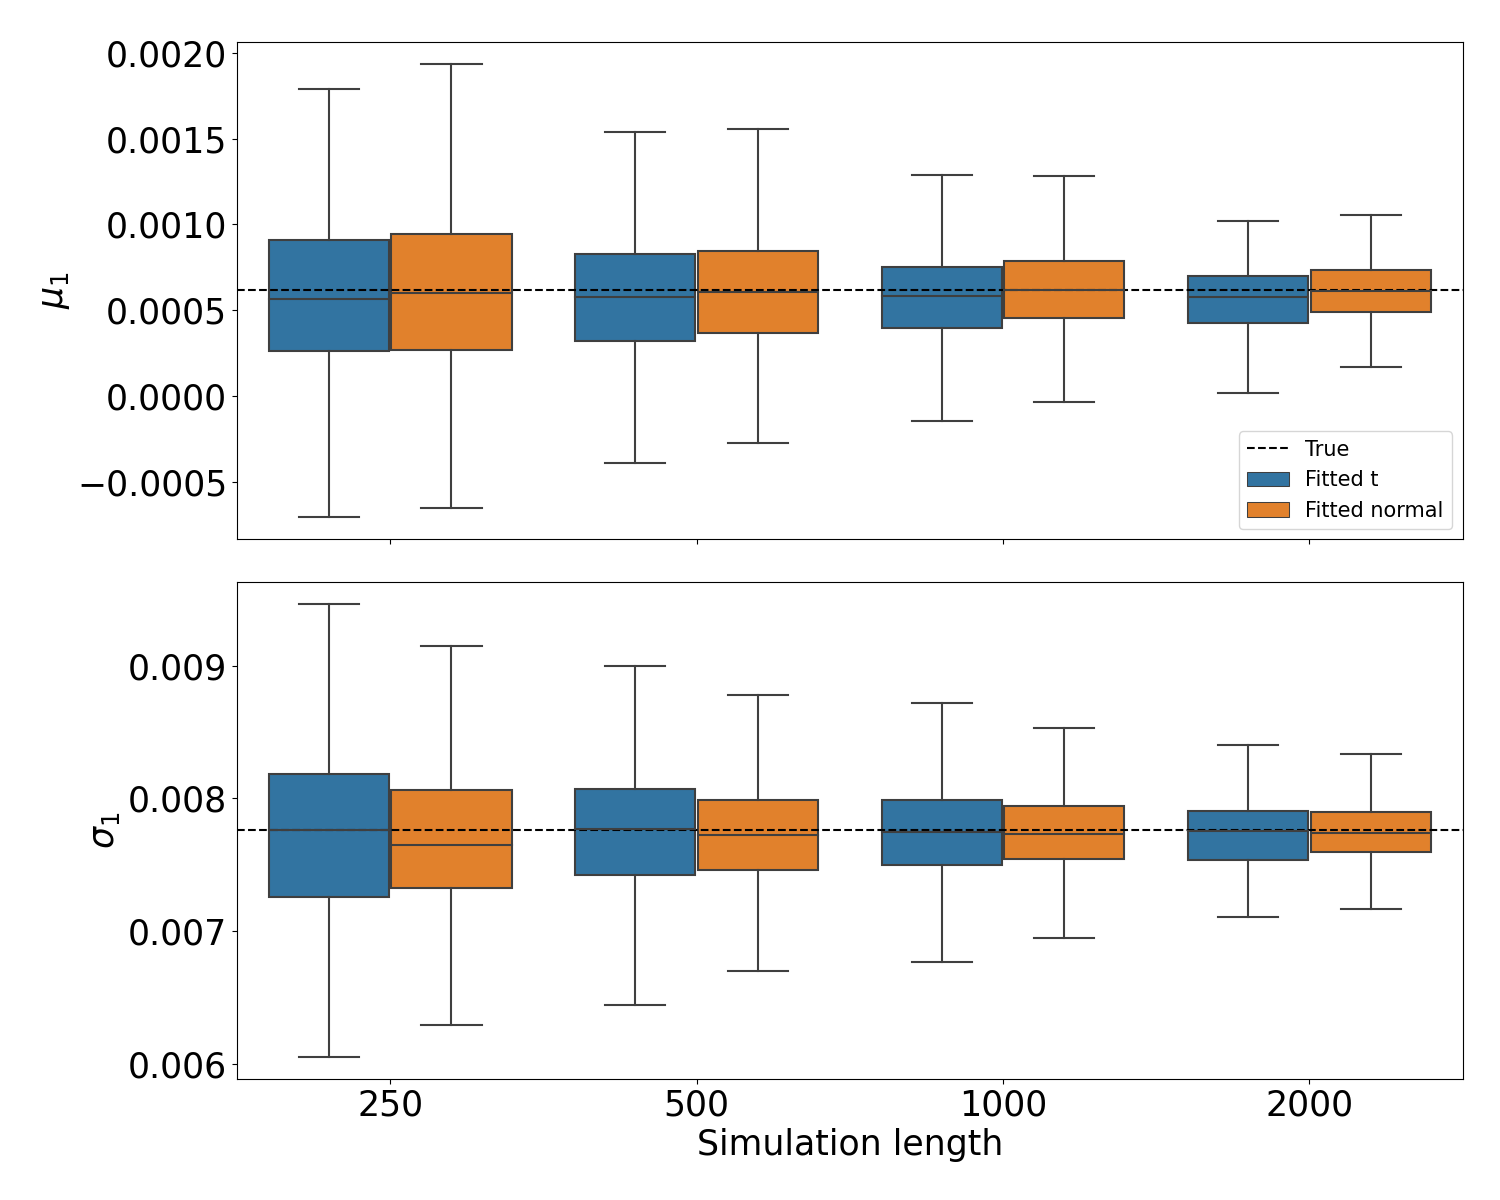
\includegraphics[width=1\textwidth]{analysis/model_convergence/images/theoretical_fit_t_dist.png}
    \caption[Empirical fit of a normal and t-distribution to data simulated from a t-distribution with five degrees of freedom]{Empirical fit of a normal and t-distribution to data simulated from a t distribution with five degrees of freedom. Results are based on 1000 simulated series.}
    \label{fig:jump_theoretical_fit}
\end{figure}

\section{Reproducing TP1 and TP4}
\label{appendix:sign_rt}

\begin{figure}[H] 
    \centering
    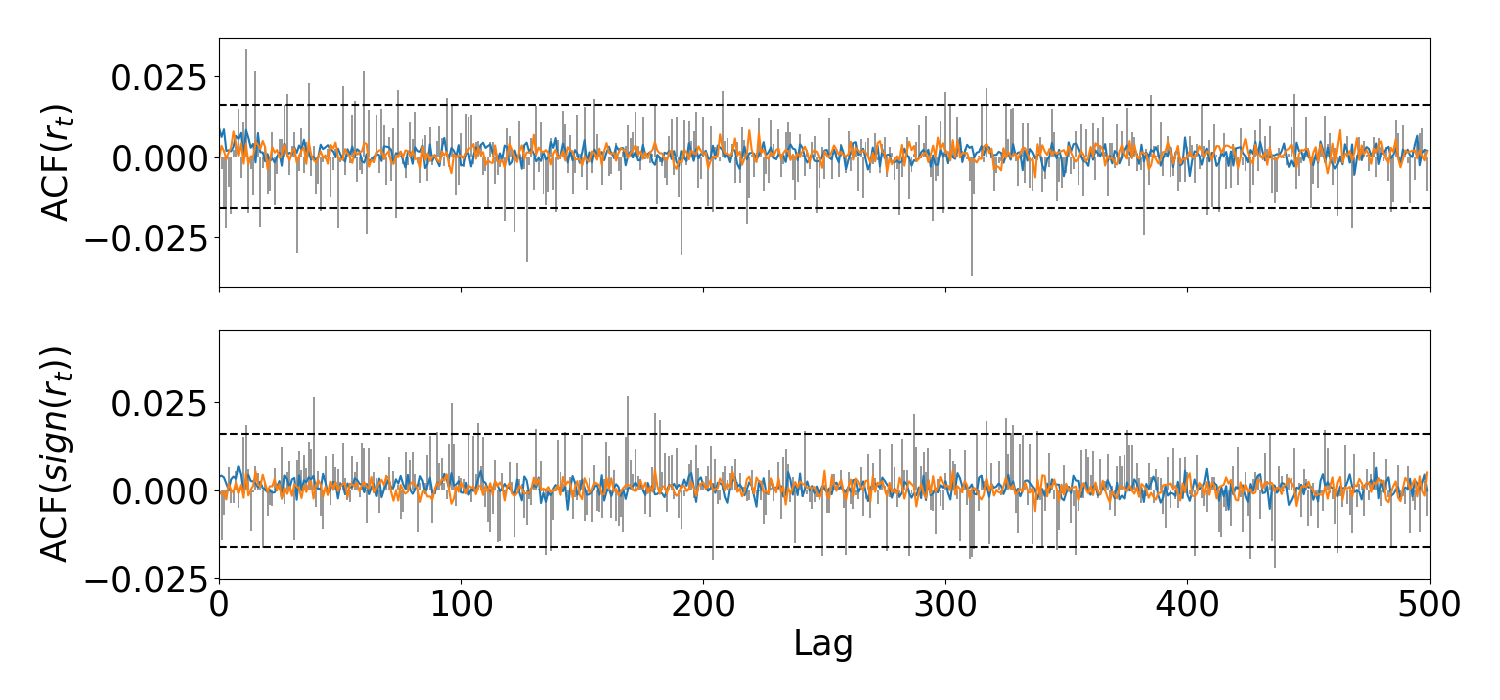
\includegraphics[width=1.0\textwidth]{analysis/stylized_facts/images/acf_sign.png}
    \caption[Autocorrelation function of $r_t$ and $sign(r_t)$]{Autocorrelation function of $r_t$ and $sign(r_t)$.}
    \label{fig:stylized_facts_acf_sign_rt} 
\end{figure}

\section{Outlier corrected rolling moments and ACF plots}

\begin{figure}[H] 
    \centering
    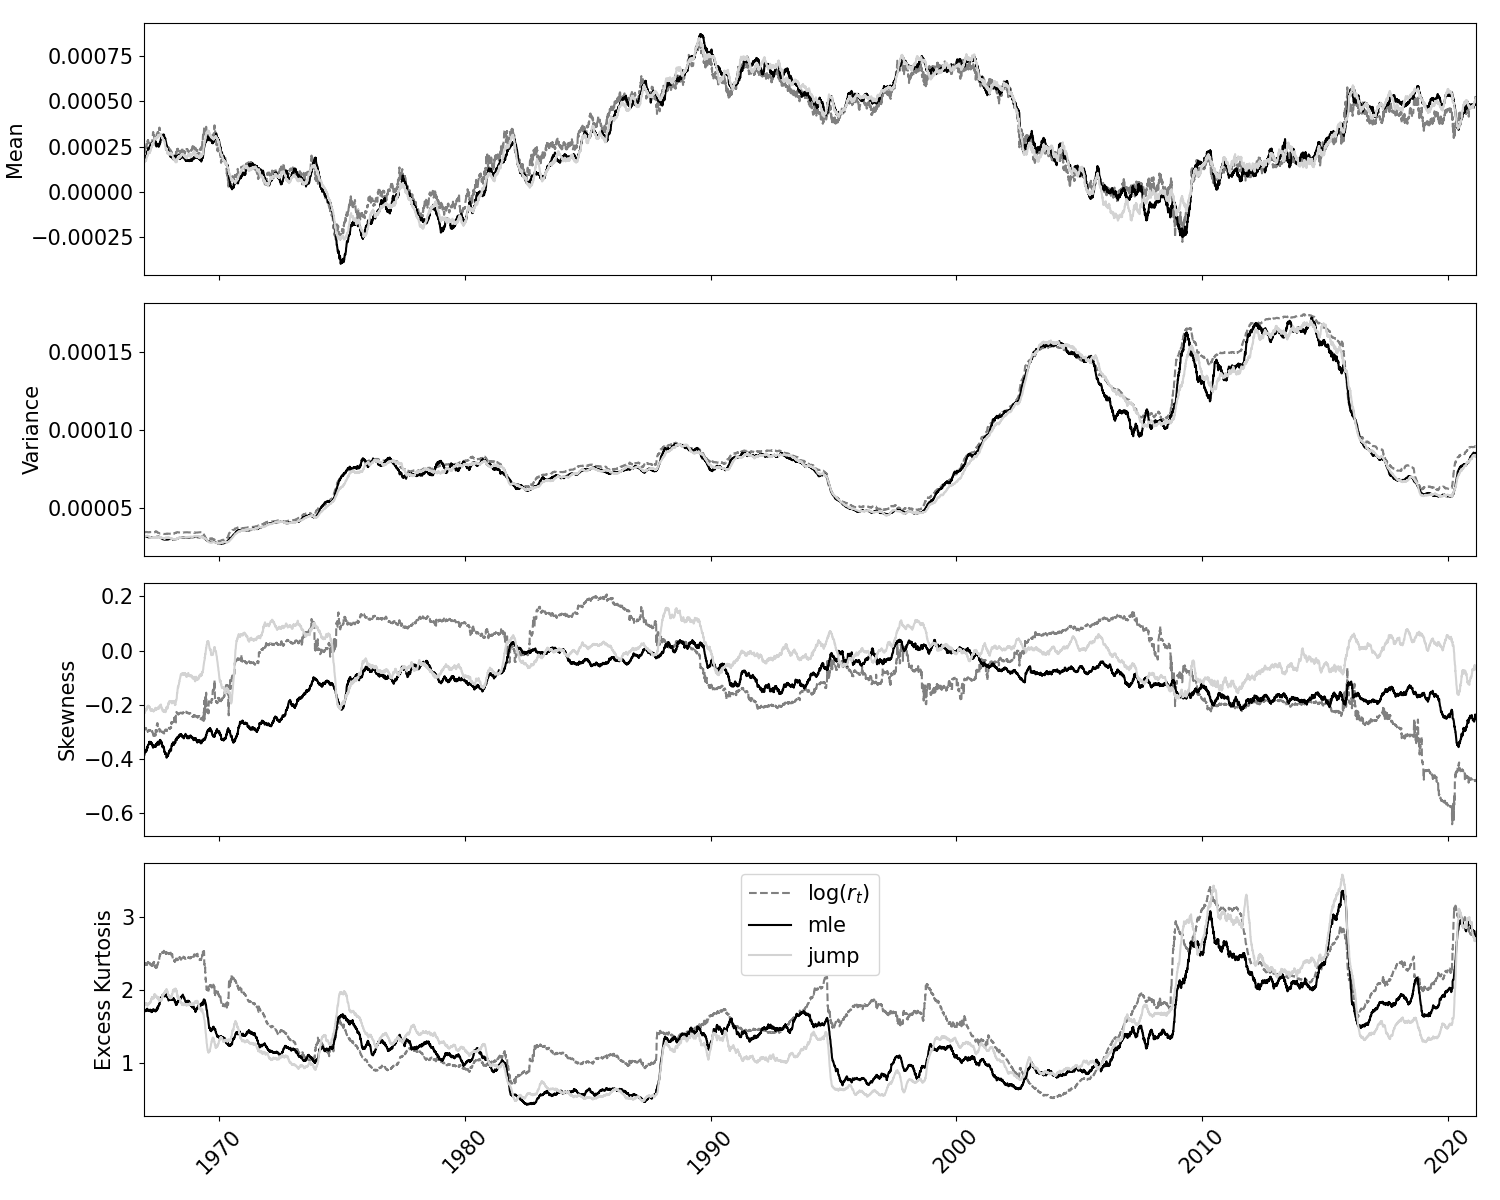
\includegraphics[width=1.0\textwidth]{analysis/stylized_facts/images/moments_outlier_corrected.png}
    
    
    \caption[Development of the first four moments from the estimated models and $r_t$]{Development of first four moments from the estimated models compared to $r_t$ using a rolling window of 1700 days. Model estimates are calculated using Monte-Carlo simulations.}
    
    \caption[Development of the first four moments from the outlier corrected estimated models and $r_t$]{Development of first four moments from the estimated models compared to $r_t$ using a rolling window of 1700 days. Model estimates are calculated using Monte-Carlo simulations correcting for outliers that are further than four standard deviations away from the mean. Outliers are treated locally in each subsample of 1700 observations.}
\label{fig:stylized_facts_rolling_moments_outliers_appendix}
\end{figure}

\begin{figure}[H] 
    \centering
    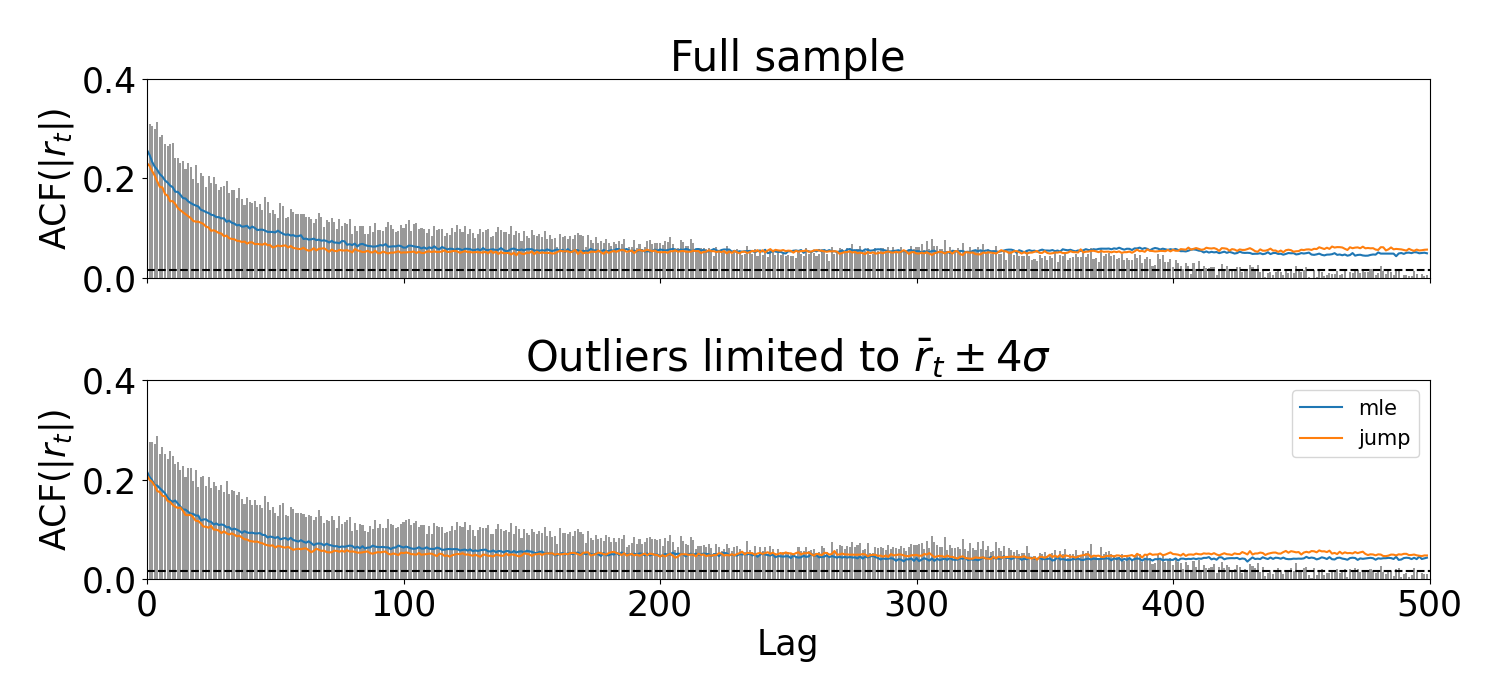
\includegraphics[width=1.0\textwidth]{analysis/stylized_facts/images/acf_abs_outlier.png}
    \caption[Autocorrelation function of $|r_t|$]{Autocorrelation function of $|r_t|$. The panel shows results on the full data and the bottom panel shows results after correcting outliers to $\bar r_t \pm 4\sigma$.}
\label{fig:stylized_facts_acf_abs_outlier}
\end{figure}


From the \cref{fig:stylized_facts_acf_plots_sub_periods}, it is evident that the autocorrelation functions estimated directly from the \mle and \jump model show a much faster decay than the decay of the empirical absolute ACF, thereby confirming the results of both Rýden et al (1998) and Bulla et al. (2011). Despite this property, the autocorrelation function generated by both the \mle and \jump model, does capture the general tendency of the empirical absolute ACF reasonably well, with the exception of the models in sub-period 9 and 10. However, it also appears that the \jump model provide a better fit compared to the model which is estimated through the \mle approach. This is in line with the fact that Bulla et al. (2011) concluded that t-distributed HMMs estimated by the \mle approach provide a superior fit compared to a traditional Gaussian HMM. Even though the thesis neglect the fitting of a t-distribution, the general conclusion that constraining the models either through distributional properties or jump penalizers provide a better fit holds. The neat aspect associated with splitting the the observations of the full sample absolute autocorrelation of the log returns into smaller digestable sub-periods is that the time-varying nature of the absolute autocorrelation of the empirical log returns becomes visible. As such, it appears that the long memory property associated with financial returns is better captured by splitting the full sample data into sub-periods, which in this case is 10. As such, figure \ref{fig:stylized_facts_acf_plots_sub_periods} points towards a similar conclusion as figure \ref{fig:stylized_facts_acf_plots}, since both the \mle and \jump methodology, in general, reproduces volatility clustering quite well. However, there are periods in which the models, and their associated parameters, fail to fit the absolute ACF of the log returns, which could be due to the models being miss-specified for some time-periods due to the rolling estimation procedure as argued for figure \ref{fig: MLE estimation rolling parameters} and \ref{fig: Jump estimation rolling parameters}. 
